\documentclass[12pt]{article}
\usepackage{amsmath,graphicx,geometry}
\usepackage{fancyhdr}
\usepackage{titlesec}
\usepackage{enumitem}
\usepackage{caption}
\usepackage{subcaption}
\usepackage{float}
\geometry{margin=1in}
\pagestyle{fancy}
\fancyhf{}
\rhead{April 6, 2025}
\lhead{DIGITAL SIGNAL PROCESSING (SPRING 2024-25)}
\rfoot{Page \thepage}

\titleformat{\section}{\large\bfseries}{\thesection}{1em}{}
\titleformat{\subsection}{\normalsize\bfseries}{\thesubsection}{1em}{}

\title{\textbf{FIR FILTER DESIGN}}
\author{Student Roll Number: 22B3954 \\
Name: Hardik Khariwal \\
Filter Number: 79}
\date{}

\begin{document}

\maketitle
\thispagestyle{fancy}

\tableofcontents
\newpage

\section{Problem Statement}
Construct a discrete time filter which allows frequencies in two different bands. The filter is an FIR Multi-Band pass Filter. Bandpass filters have transition bands of 5kHz on either side of each passband. Both passband and stopband are monotonic. Bandstop filters have transition bands of 5kHz on either side of each stopband. The filter magnitude response has passband and stopband tolerances of 0.15 each. The given signal is bandlimited to 280 kHz and ideally sampled at 600 kHz.

\section{Preliminaries}
The filter number assigned: \( M = 39 \)

\[
M = 11Q + R \Rightarrow Q = 7, R = 2
\]

The passband frequency ranges (in kHz) are given in two groups (for parameter D):

\begin{itemize}
    \item Group I: (40 + 5D) to (70 + 5D), where \( D = Q \)
    \item Group II: (170 + 5D) to (200 + 5D), where \( D = R \)
\end{itemize}

Therefore, the passband ranges are:
\begin{itemize}
    \item 75 kHz to 105 kHz
    \item 180 kHz to 210 kHz
\end{itemize}

Sampling rate is 630 kHz. Hence, the maximum frequency component is 280 kHz.

This filter is implemented using a \textbf{parallel cascade} structure:
\begin{itemize}
    \item A bandpass filter with a passband from 75 kHz to 105 kHz
    \item A bandpass filter with a passband from 180 kHz to 210 kHz
\end{itemize}

The final FIR filter is obtained by summing the outputs of these two bandpass filters. This configuration allows the filter to pass two distinct frequency bands while attenuating all others.


\section{Band-Pass Filter:Group-1}
\subsection{Unnormalized Discrete Time Filter Specifications}
\begin{enumerate}
    \item Passband: 75 to 105 kHz
    \item Stopband: 0 to 70 kHz and 110 to 280 kHz
    \item Passband Tolerance: 0.15
    \item Stopband Tolerance: 0.15
\end{enumerate}

\subsection{Normalized Discrete Time Filter Specifications}
Sampling rate = 630 kHz. On the normalized frequency axis, the sampling rate corresponds to \( 2\pi \). Therefore, any frequency can be normalized as:

\[
\omega = \frac{\Omega \cdot 2\pi}{\Omega_s}
\]

\[
\omega_{c1} = \frac{(f_{s1} + f_{p1}) \cdot 2\pi}{2 \cdot f_{\text{samp}}}
= \frac{(70\,\text{kHz} + 75\,\text{kHz}) \cdot 2\pi}{2 \cdot 630\,\text{kHz}}
= 0.575\,\text{rad}
\]

\[
\omega_{c2} = \frac{(f_{p2} + f_{s2}) \cdot 2\pi}{2 \cdot f_{\text{samp}}}
= \frac{(105\,\text{kHz} + 110\,\text{kHz}) \cdot 2\pi}{2 \cdot 630\,\text{kHz}}
= 0.861\,\text{rad}
\]


\begin{itemize}
    \item Passband: \(0.723\,\text{rad}\) to \(1.072\,\text{rad}\)
    \item Stopband: \(0\) to \(0.723\,\text{rad}\) and \(1.072\,\text{rad}\) to \(\pi\,\text{rad}\)
\end{itemize}


\subsection{Designing FIR Band-pass}
Given \( \delta = 0.15 \):

\[
A = -20 \log_{10}(\delta) = 16.478 \, \text{dB}
\]

\[
\beta =
\begin{cases}
0, & \text{if } A < 21 \\
0.5842 \cdot (A - 21)^{0.4} + 0.07886 \cdot (A - 21), & \text{if } 21 \leq A < 51 \\
0.1102 \cdot (A - 8.7), & \text{if } A \geq 51
\end{cases}
\]
Since \( A < 21 \), we use:
\[
\beta = 0
\]

The transition bandwidth is calculated as:
\[
\Delta \omega_T = \frac{5 \times 10^3 \cdot 2\pi}{630 \times 10^3} = 0.0159\pi
\]

Using the empirical formula for minimum filter order:
\[
2N \geq \frac{A - 7.95}{2.285 \cdot \Delta \omega_T} = \frac{16.4782}{2.285 \cdot 0.0159\pi} \approx 145.75 \Rightarrow N \approx 74
\]

Rounding up:
\[
N_{\text{min}} = 74
\]

Using trial and error for optimal performance, we finally select:
\[
N = 99
\]


The time domain coefficients were obtained by:
\begin{itemize}
    \item Generating ideal impulse responses of two LPFs
    \item Subtracting them to get BPF
    \item Applying Kaiser Window using MATLAB
\end{itemize}

\subsection{Figures}

\begin{figure}[H]
    \centering
    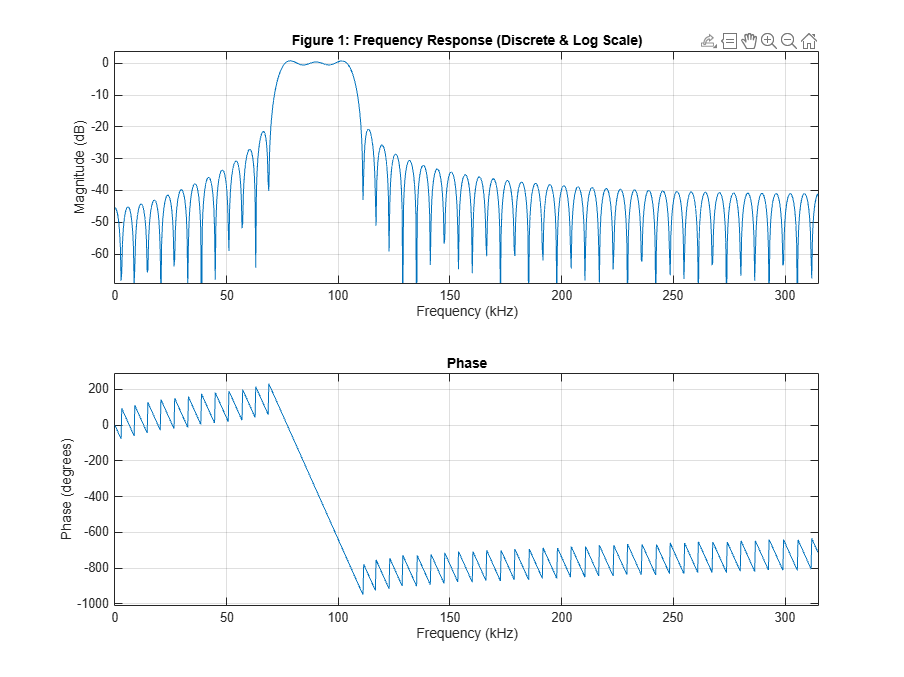
\includegraphics[height=13cm]{g11.png}
    \caption{Frequency Response (Discrete and Log Scale)}
    \label{fig:freq_response}
\end{figure}

\begin{figure}[H]
    \centering
    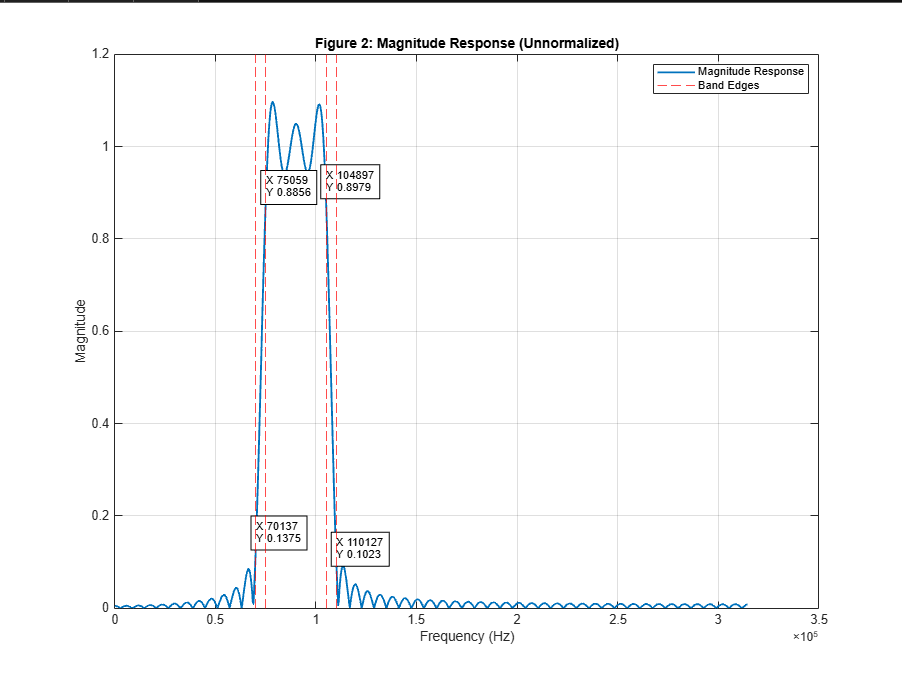
\includegraphics[height=13cm]{g18.png}
    \caption{Magnitude Response (Unnormalized)}
    \label{fig:mag_response}
\end{figure}

\begin{figure}[H]
    \centering
    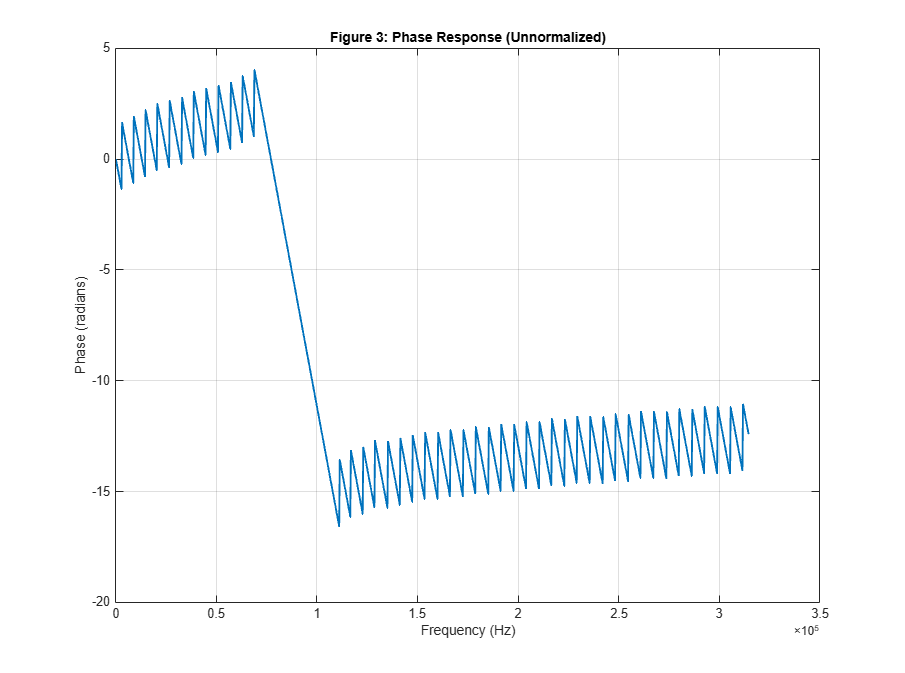
\includegraphics[height=13cm]{g13.png}
    \caption{Phase Response (Unnormalized)}
    \label{fig:phase_response}
\end{figure}

\begin{figure}[H]
    \centering
    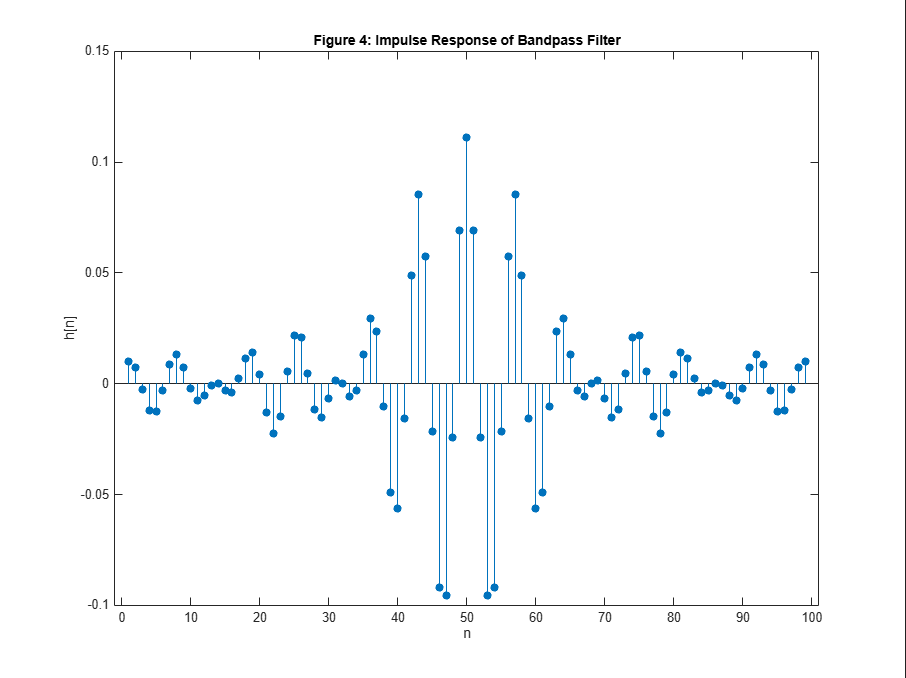
\includegraphics[height=13cm]{g14.png}
    \caption{Impulse Response of Bandpass Filter}
    \label{fig:impulse_response}
\end{figure}

\begin{figure}[H]
    \centering
    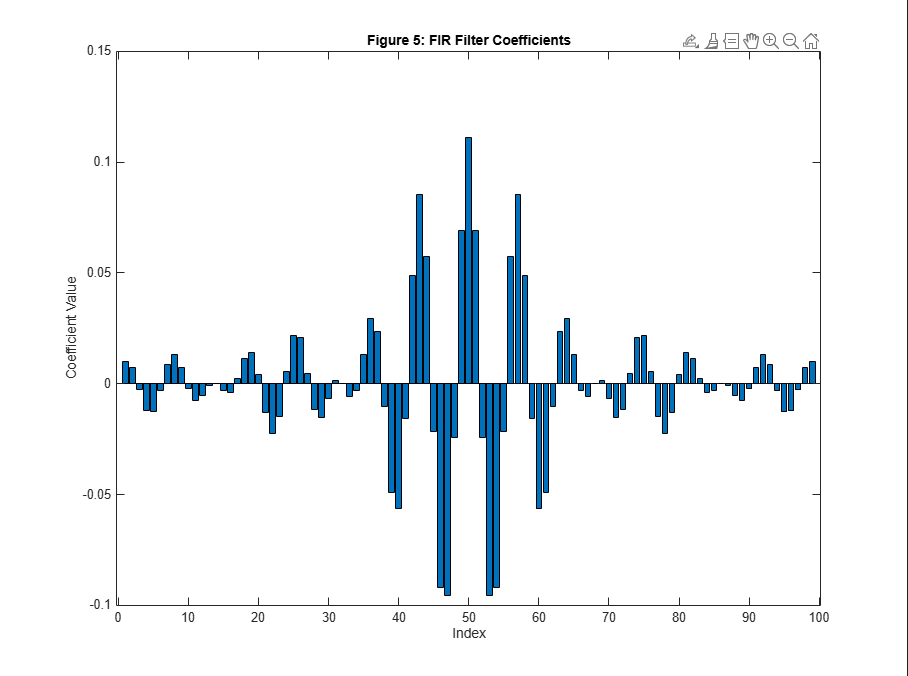
\includegraphics[height=13cm]{g15.png}
    \caption{FIR Filter Coefficients}
    \label{fig:coefficients}
\end{figure}

\begin{figure}[H]
    \centering
    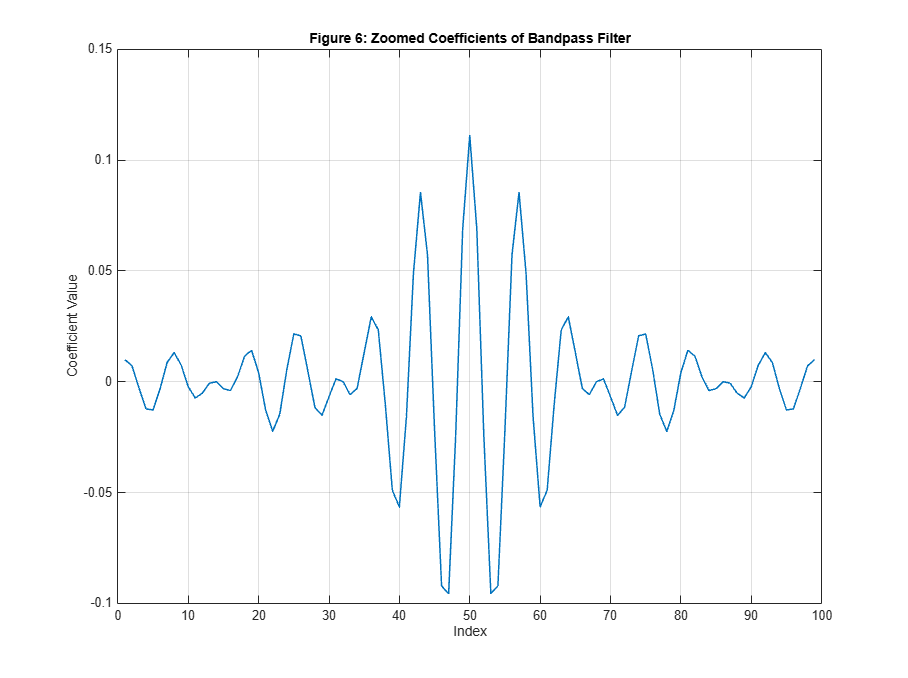
\includegraphics[height=13cm]{g16.png}
    \caption{Zoomed Coefficients of Bandpass Filter}
    \label{fig:zoomed_coefficients}
\end{figure}

\begin{figure}[H]
    \centering
    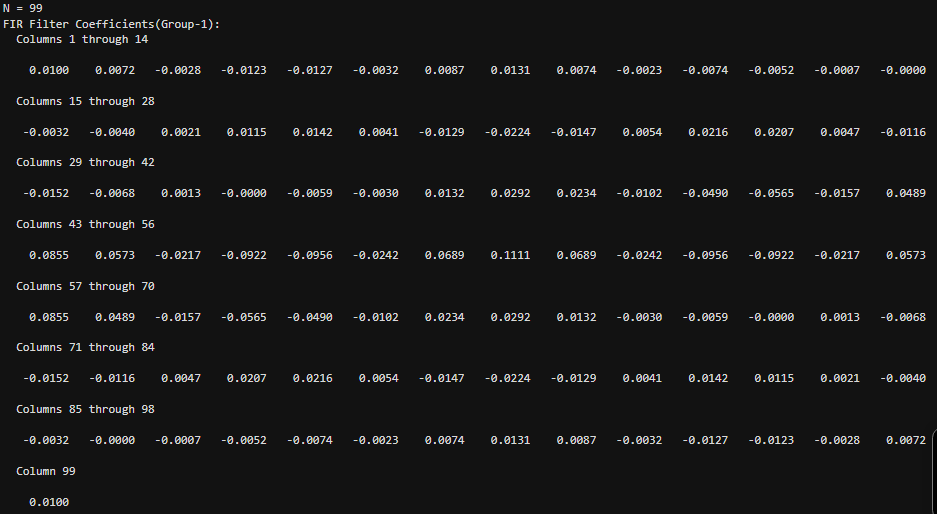
\includegraphics[height=10cm]{g19.png}
    \caption{BandPass Impulse Response Value (Group1)}
    \label{fig:fir_coefficients_g1}
\end{figure}

\section{Band-Pass Filter:Group-2}
\subsection{Unnormalized Discrete Time Filter Specifications}
\begin{enumerate}
    \item Passband: 180 to 210 kHz
    \item Stopband: 0 to 175 kHz and 215 to 280 kHz
    \item Passband Tolerance: 0.15
    \item Stopband Tolerance: 0.15
\end{enumerate}

\subsection{Normalized Discrete Time Filter Specifications}
Sampling rate = 630 kHz. On the normalized frequency axis, the sampling rate corresponds to \( 2\pi \). Therefore, any frequency can be normalized as:

\[
\omega = \frac{\Omega \cdot 2\pi}{\Omega_s}
\]

\[
\omega_{c1} = \frac{(f_{s1} + f_{p1}) \cdot 2\pi}{2 \cdot f_{\text{samp}}}
= \frac{(175\,\text{kHz} + 180\,\text{kHz}) \cdot 2\pi}{2 \cdot 630\,\text{kHz}}
= 1.770\,\text{rad}
\]

\[
\omega_{c2} = \frac{(f_{p2} + f_{s2}) \cdot 2\pi}{2 \cdot f_{\text{samp}}}
= \frac{(210\,\text{kHz} + 215\,\text{kHz}) \cdot 2\pi}{2 \cdot 630\,\text{kHz}}
= 2.119\,\text{rad}
\]

\begin{itemize}
    \item Passband: \(1.770\,\text{rad}\) to \(2.119\,\text{rad}\)
    \item Stopband: \(0\) to \(1.770\,\text{rad}\) and \(2.119\,\text{rad}\) to \(\pi\,\text{rad}\)
\end{itemize}

\subsection{Designing FIR Band-pass}
Given \( \delta = 0.15 \):

\[
A = -20 \log_{10}(\delta) = 16.478 \, \text{dB}
\]

\[
\beta =
\begin{cases}
0, & \text{if } A < 21 \\
0.5842 \cdot (A - 21)^{0.4} + 0.07886 \cdot (A - 21), & \text{if } 21 \leq A < 51 \\
0.1102 \cdot (A - 8.7), & \text{if } A \geq 51
\end{cases}
\]
Since \( A < 21 \), we use:
\[
\beta = 0
\]

The transition bandwidth is calculated as:
\[
\Delta \omega_T = \frac{5 \times 10^3 \cdot 2\pi}{630 \times 10^3} = 0.0159\pi
\]

Using the empirical formula for minimum filter order:
\[
2N \geq \frac{A - 7.95}{2.285 \cdot \Delta \omega_T} = \frac{16.4782}{2.285 \cdot 0.0159\pi} \approx 147.63 \Rightarrow N \approx 75
\]

Rounding up:
\[
N_{\text{min}} = 75
\]

Using trial and error for optimal performance, we finally select:
\[
N = 95
\]

The time domain coefficients were obtained by:
\begin{itemize}
    \item Generating ideal impulse responses of two LPFs
    \item Subtracting them to get BPF
    \item Applying Kaiser Window using MATLAB
\end{itemize}

\subsection{Figures}

\begin{figure}[H]
    \centering
    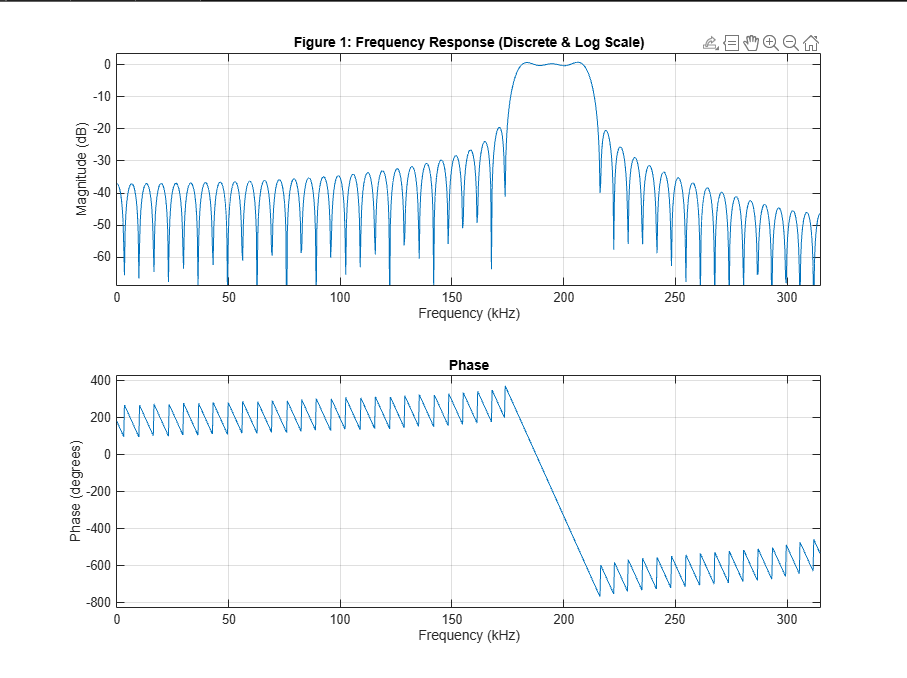
\includegraphics[height=13cm]{g21.png}
    \caption{Frequency Response (Discrete and Log Scale)}
    \label{fig:freq_response_g2}
\end{figure}

\begin{figure}[H]
    \centering
    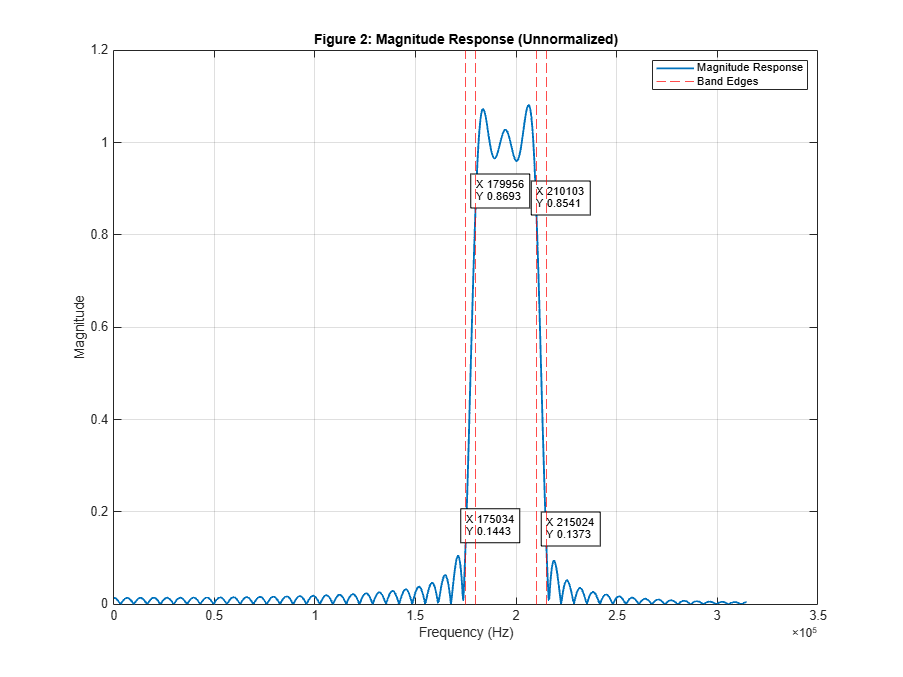
\includegraphics[height=13cm]{g28.png}
    \caption{Magnitude Response (Unnormalized)}
    \label{fig:mag_response_g2}
\end{figure}

\begin{figure}[H]
    \centering
    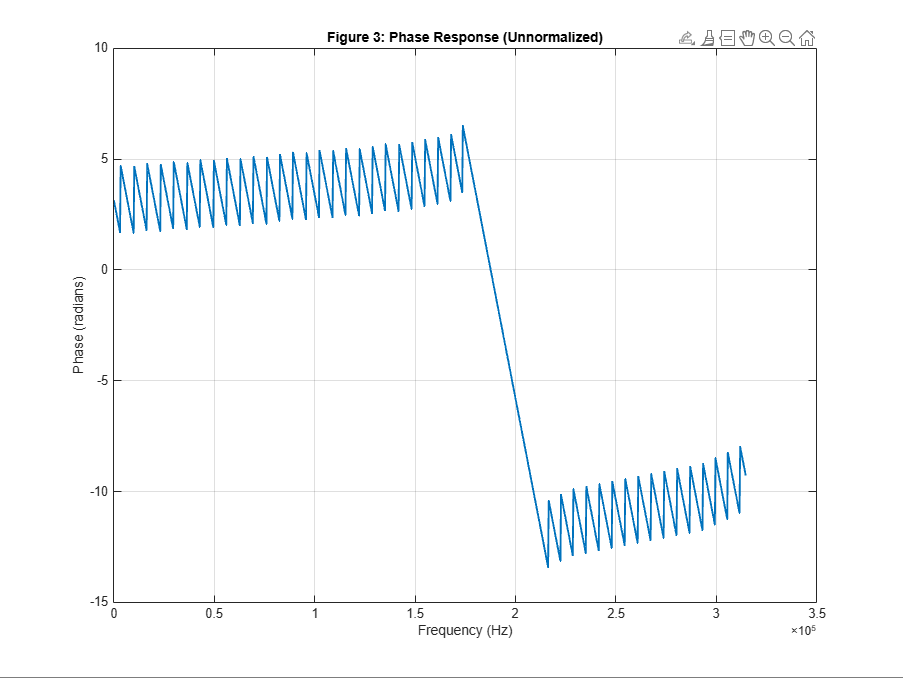
\includegraphics[height=13cm]{g23.png}
    \caption{Phase Response (Unnormalized)}
    \label{fig:phase_response_g2}
\end{figure}

\begin{figure}[H]
    \centering
    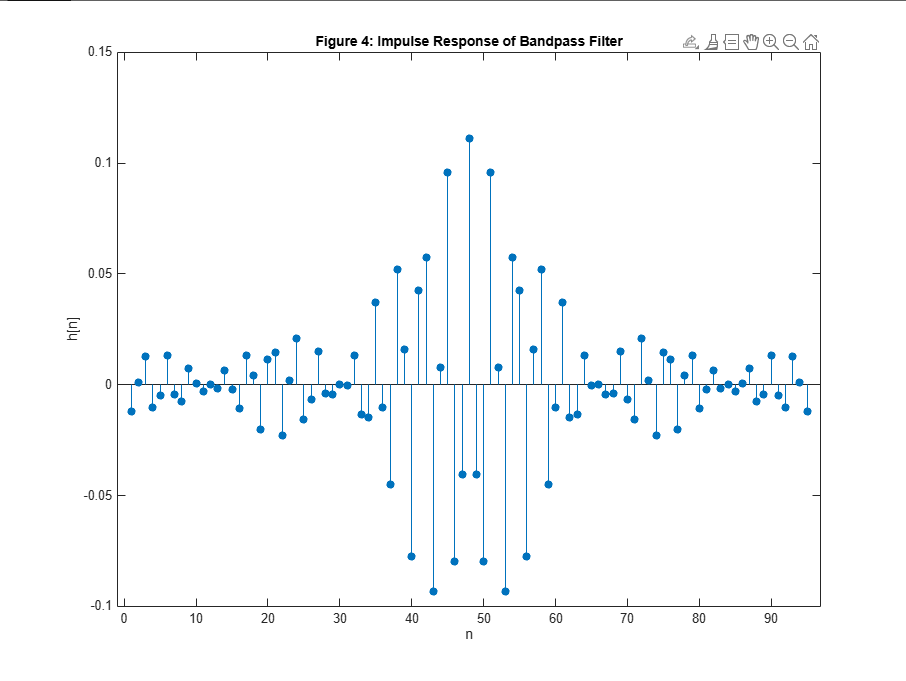
\includegraphics[height=13cm]{g24.png}
    \caption{Impulse Response of Bandpass Filter}
    \label{fig:impulse_response_g2}
\end{figure}

\begin{figure}[H]
    \centering
    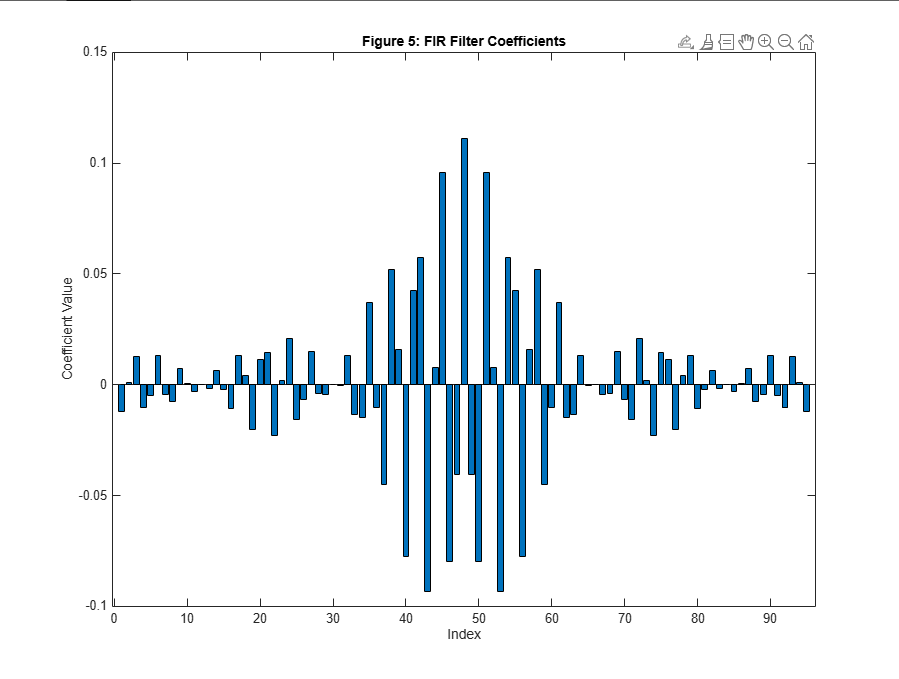
\includegraphics[height=13cm]{g25.png}
    \caption{FIR Filter Coefficients}
    \label{fig:coefficients_g2}
\end{figure}

\begin{figure}[H]
    \centering
    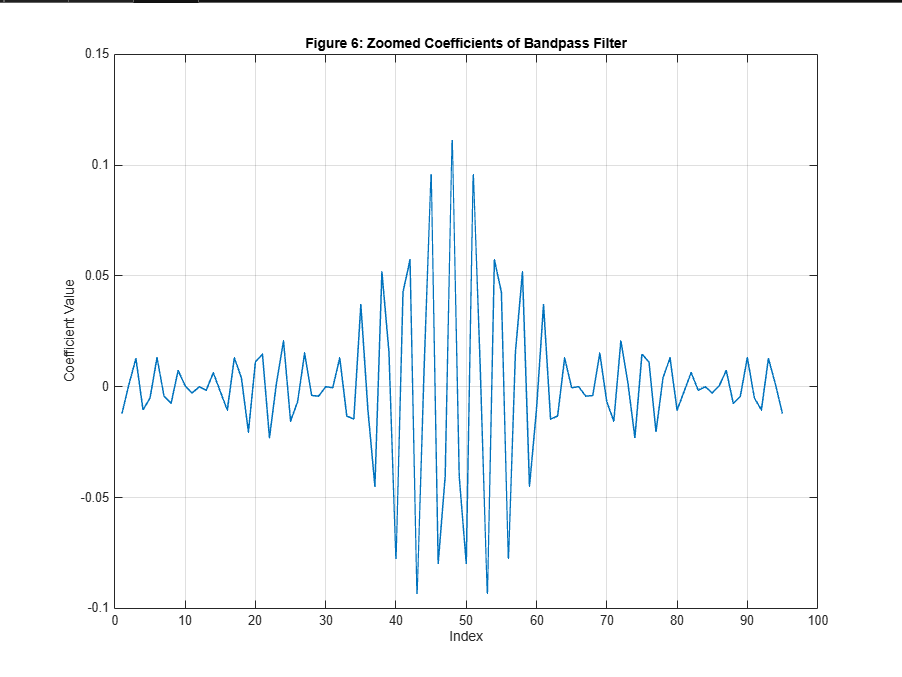
\includegraphics[height=13cm]{g26.png}
    \caption{Zoomed Coefficients of Bandpass Filter}
    \label{fig:zoomed_coefficients_g2}
\end{figure}

\begin{figure}[H]
    \centering
    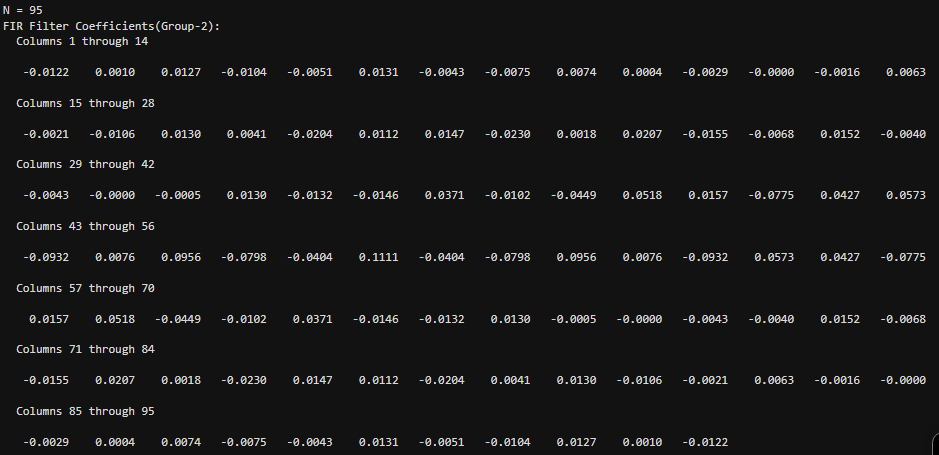
\includegraphics[height=9cm]{g29.png}
    \caption{BandPass Impulse Response Value (Group2)}
    \label{fig:fir_coefficients_g2}
\end{figure}


\section{Net Filter Response}
The final FIR filter is designed using the parallel method by combining two separate FIR band-pass filters:

\begin{itemize}
    \item \textbf{Group 1 (G1):} Band-pass filter from 75 kHz to 105 kHz
    \item \textbf{Group 2 (G2):} Band-pass filter from 180 kHz to 210 kHz
\end{itemize}

The two filters are added in parallel to create a multiband FIR filter. 

As a result, the final filter allows the following frequency bands to pass:
\begin{itemize}
    \item 75 kHz to 105 kHz
    \item 180 kHz to 210 kHz
\end{itemize}
\subsection{Final Net Multiband Pass FIR Filter Results}

\begin{figure}[H]
    \centering
    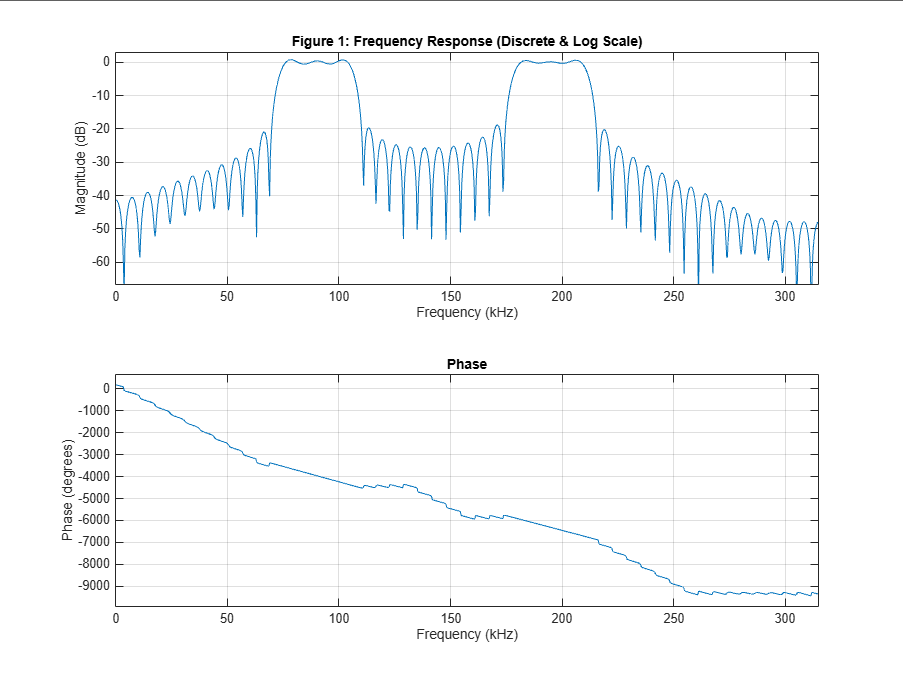
\includegraphics[height=13cm]{1.png}
    \caption{Frequency Response (Discrete and Logarithmic Scale) of Final Multiband FIR Filter}
    \label{fig:final_freq_response}
\end{figure}

\begin{figure}[H]
    \centering
    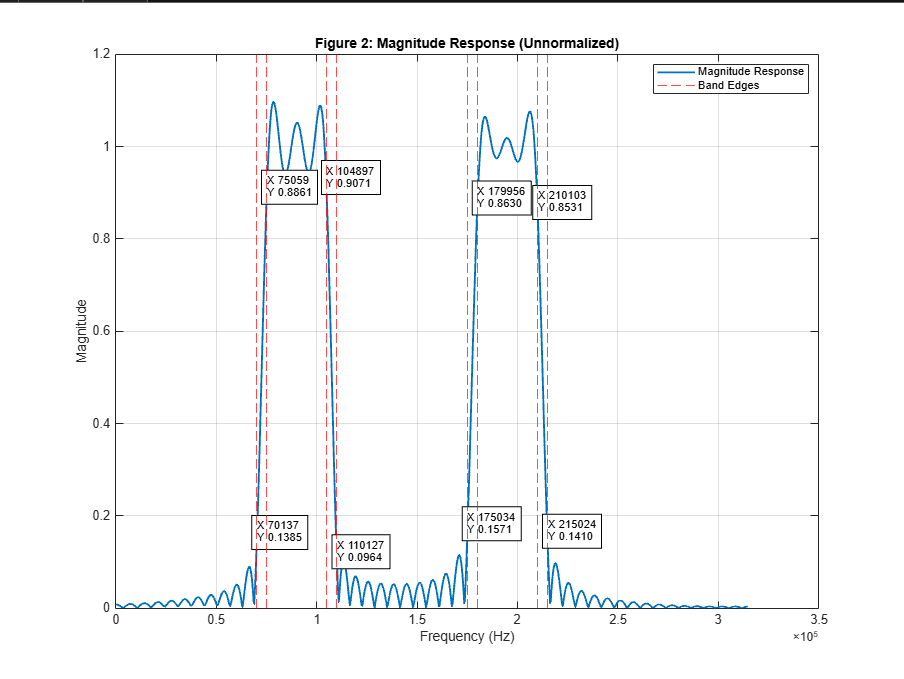
\includegraphics[height=13cm]{2.png}
    \caption{Unnormalized Magnitude Response of Final FIR Filter}
    \label{fig:final_mag_response}
\end{figure}

\begin{figure}[H]
    \centering
    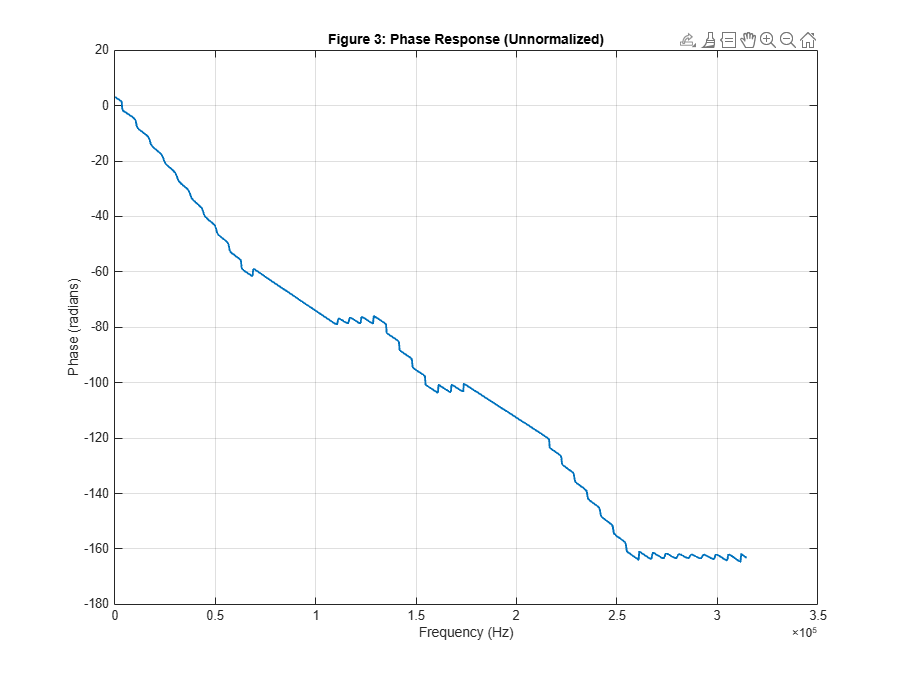
\includegraphics[height=13cm]{3.png}
    \caption{Unnormalized Phase Response of Final FIR Filter}
    \label{fig:final_phase_response}
\end{figure}

\begin{figure}[H]
    \centering
    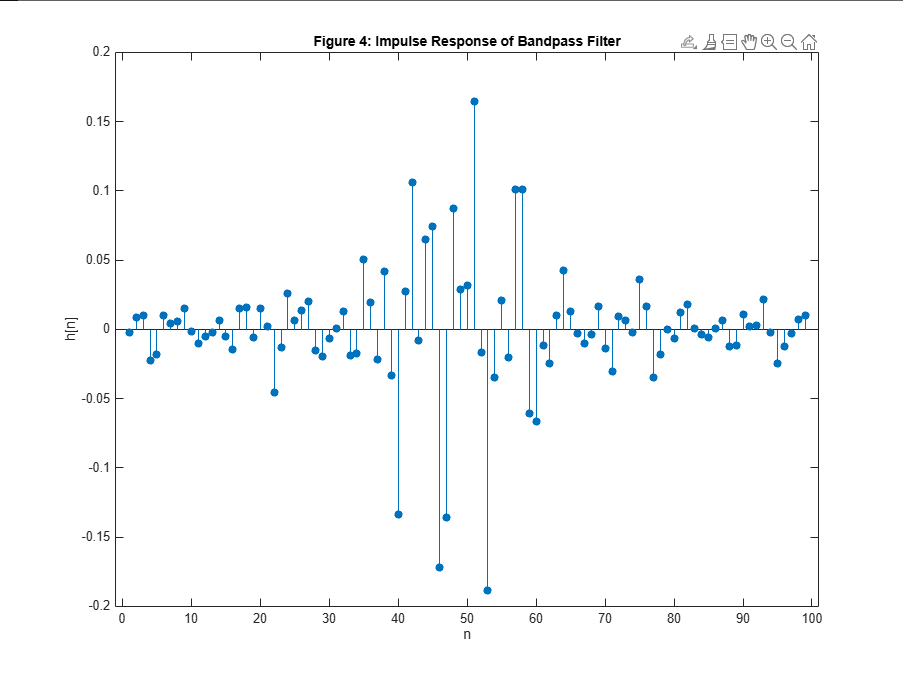
\includegraphics[height=13cm]{4.png}
    \caption{Impulse Response of Final Multiband Bandpass FIR Filter}
    \label{fig:final_impulse_response}
\end{figure}

\begin{figure}[H]
    \centering
    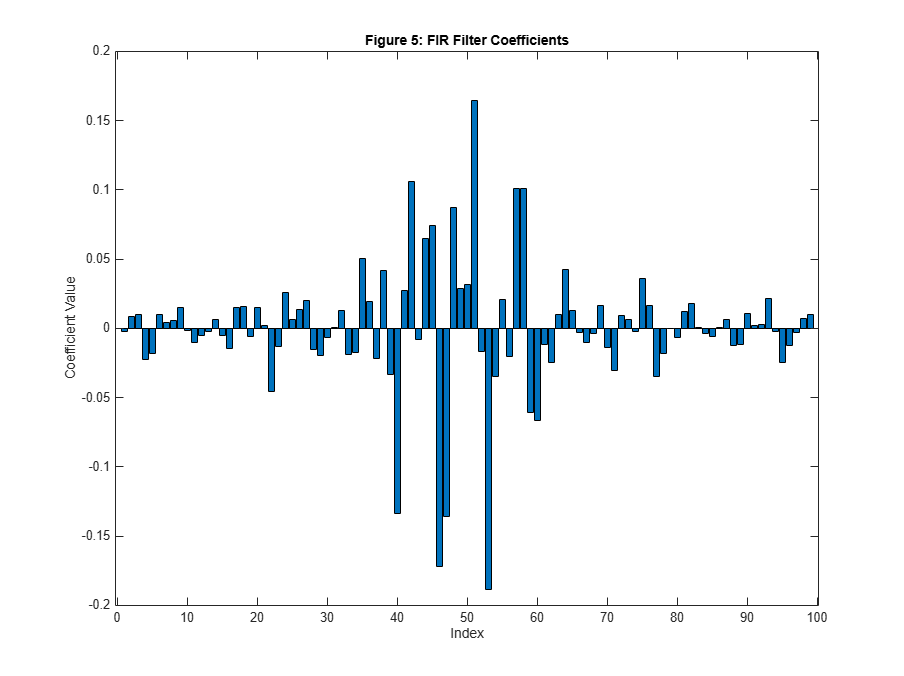
\includegraphics[height=13cm]{5.png}
    \caption{FIR Filter Coefficients of Final Multiband Filter}
    \label{fig:final_coefficients}
\end{figure}

\begin{figure}[H]
    \centering
    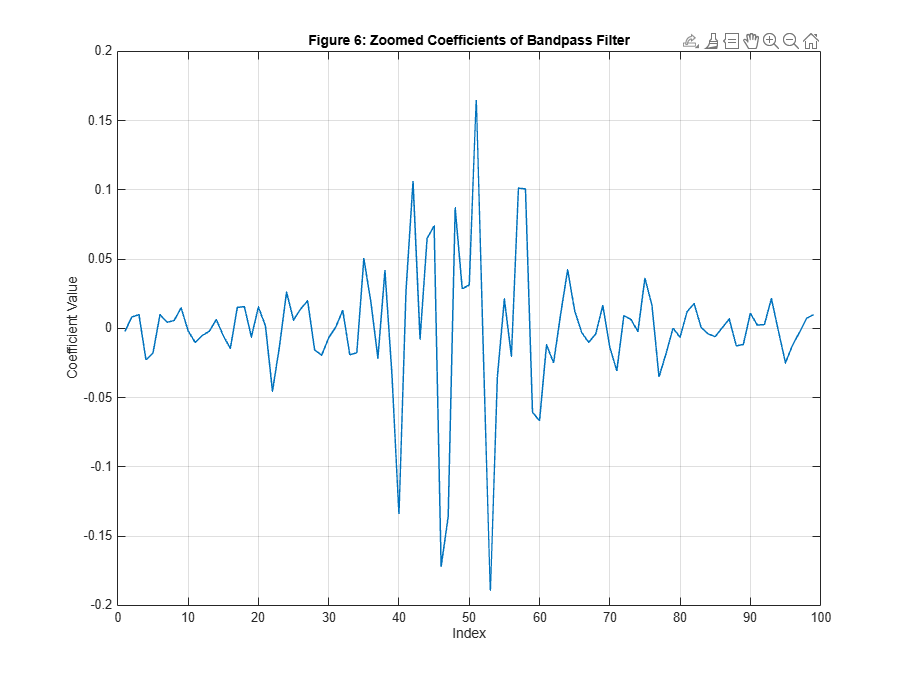
\includegraphics[height=13cm]{6.png}
    \caption{Zoomed View of FIR Filter Coefficients}
    \label{fig:final_zoomed_coefficients}
\end{figure}

\begin{figure}[H]
    \centering
    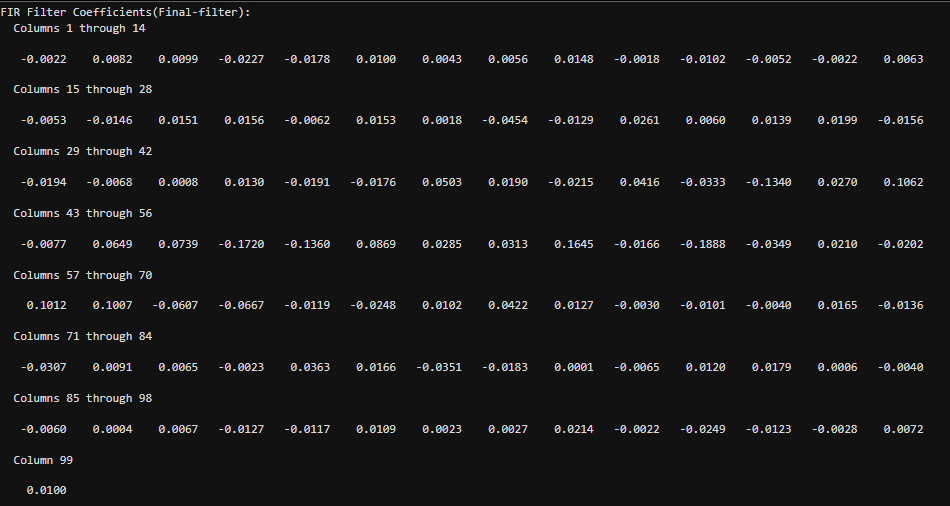
\includegraphics[height=9cm]{7.png}
    \caption{Impulse Response Value Detail for Final Multiband FIR Filter}
    \label{fig:final_impulse_detail}
\end{figure}

\subsection{Magnitude Response at Key Frequencies}

\begin{table}[H]
    \centering
    \begin{tabular}{|c|c|}
        \hline
        \textbf{Frequency (Hz)} & \textbf{Magnitude} \\
        \hline
        70,000   & 0.1385 \\
        75,000   & 0.8861 \\
        105,000  & 0.9071 \\
        110,000  & 0.0964 \\
        175,000  & 0.1471 \\
        180,000  & 0.8630 \\
        210,000  & 0.8531 \\
        215,000  & 0.1410 \\
        \hline
    \end{tabular}
    \caption{Measured Magnitudes at Critical Frequencies for Final FIR Filter}
    \label{tab:magnitude_values}
\end{table}






\subsection{Comparison with IIR Filter from Mid-Semester Exam}

The final multiband FIR filter design differs from the IIR filter implemented during the mid-semester take-home component in the following ways:

\begin{itemize}
    \item \textbf{Filter Type:} The FIR filter is non-recursive and uses a finite impulse response, while the IIR filter is recursive with infinite impulse response.
    \item \textbf{Stability:} FIR filters are inherently stable. The IIR filter required careful pole placement to ensure stability.
    \item \textbf{Phase Response:} The FIR filter has a linear phase, making it suitable for applications requiring phase preservation. The IIR filter had a nonlinear phase response.
    \item \textbf{Computational Complexity:} The FIR filter has higher computational complexity due to more coefficients, while the IIR filter achieved similar performance with fewer coefficients.
    \item \textbf{Group Delay:} FIR filters introduce more delay because of the longer impulse response. The IIR filter had lower group delay.
    \item \textbf{Implementation:} The FIR filter used window-based design, while the IIR filter was designed using Butterworth/Chebyshev approximation and bilinear transformation.
    \item \textbf{Transition Band:} The FIR design offers sharper control in multiband regions, though at the cost of increased order. The IIR filter had broader transition bands.
\end{itemize}

\vspace{0.5cm}
\begin{figure}[H]
    \centering
    \begin{subfigure}{0.48\textwidth}
        \centering
        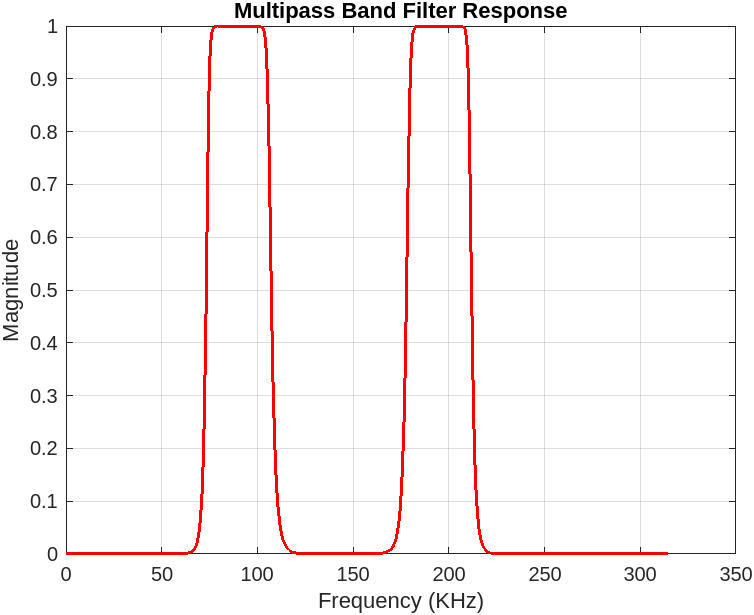
\includegraphics[height=6cm]{combined_magnitude_response.png} % Replace with actual filename
        \caption{IIR Filter Magnitude Response}
        \label{fig:iir_mag}
    \end{subfigure}
    \hfill
    \begin{subfigure}{0.48\textwidth}
        \centering
        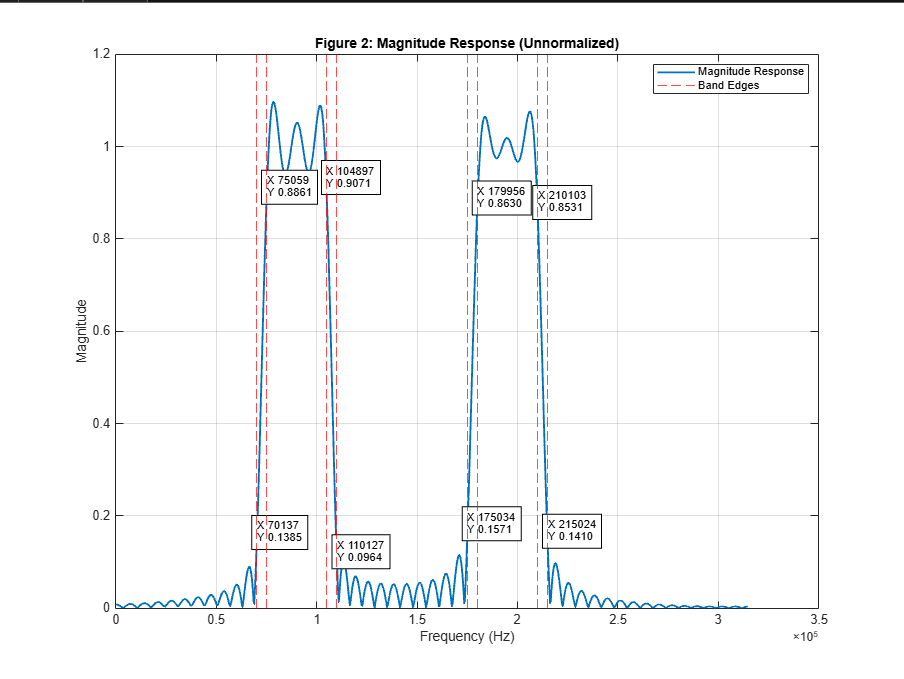
\includegraphics[height=6cm]{2.png} % Replace with actual filename
        \caption{FIR Filter Magnitude Response}
        \label{fig:fir_mag}
    \end{subfigure}
    \caption{Comparison of Magnitude Responses: IIR vs FIR Filters}
    \label{fig:iir_vs_fir}
\end{figure}

\begin{table}[H]
    \centering
    \begin{tabular}{|p{5cm}|c|c|}
        \hline
        \textbf{Criteria} & \textbf{FIR Filter} & \textbf{IIR Filter} \\
        \hline
        Filter Type & Non-recursive (FIR) & Recursive (IIR) \\
        Stability & Always Stable & Conditionally Stable \\
        Phase Response & Linear Phase & Nonlinear Phase \\
        Group Delay & Higher & Lower \\
        Magnitude Ripple & Minimal & May have ripple (Butterworth/Chebyshev) \\
        Design Method & Windowed Design & Bilinear Transform (Analog Prototype) \\
        Complexity (No. of Coefficients) & High & Low \\
        Multiband Support & Precise Band Control & Limited without high-order design \\
        \hline
    \end{tabular}
    \caption{Comparison Between Final FIR Filter and Mid-Semester IIR Filter}
    \label{tab:fir_vs_iir_comparison}
\end{table}

Overall, the FIR filter design provides better frequency control and phase characteristics at the cost of increased computational demand.

\end{document}
